\documentclass[12pt,a4paper]{report}
\usepackage[utf8]{inputenc}
\usepackage[T1]{fontenc}
\usepackage{lmodern}
\usepackage{geometry}
\usepackage{graphicx}
\usepackage{hyperref}
\usepackage{ragged2e} % Ensure full justification
\usepackage{amsmath}
\usepackage{amssymb}
\usepackage{amsfonts}
\usepackage{listings}
\lstset{
    breaklines=true,
    basicstyle=\ttfamily,
    frame=single
}
\usepackage{color}
\usepackage{fancyhdr}
\usepackage{titlesec}
\usepackage{float}
\usepackage{caption}
\usepackage{tikz}
\usepackage{tikz-qtree}
\usepackage{tikz-dependency}
\usepackage{hyperref}
\usepackage{calc}
\usepackage[noabbrev]{cleveref}
\geometry{margin=0.97in}

\newcommand{\bmr}[1]{\textcolor{red}{#1}}

\sloppy
\begin{document}
\justifying

\begin{titlepage}
    \centering
    % University Name
    {\Large \textbf{Indian Institute of Technology Kharagpur}\par}
    \vspace{0.5cm}
    % Course information
    {\Large Course Number: \textbf{CS60002}\par}
    {\Large Course Name: \textbf{Distributed Systems}\par}
    {\Large Term Project\par}
    \vspace{1cm} % Vertical space
  
    % University logo in the middle
    
\includegraphics[width=0.6\textwidth]{img/iit_kgp_logo.png}\par
    \vspace{1cm}
  
    % Student names on separate lines
    {\Large Bratin Mondal - 21CS10016\par}
    {\Large Soukhin Nayek - 21CS10062\par}
    {\Large Swarnabh Mandal - 21CS10068\par}
    \vspace{1cm}
  
    % Title of the Project
    {\Huge\bfseries Distributed Storage Service\par}
    
    \vfill
    {\Large \today\par}
\end{titlepage}

\tableofcontents
\clearpage

\chapter{Introduction}\label{chap:intro}

Distributed storage services are systems that distribute data across multiple physical nodes to ensure reliable and efficient access even in the event of hardware failures, network issues, or other disruptions. Typically, data is replicated across nodes in diverse geographical locations or data centres, which enhances scalability, performance, and overall reliability. Clients can access these systems through various interfaces, such as REST APIs or file system protocols, allowing them to store and retrieve data seamlessly from around the world. Many of these systems also incorporate mechanisms to maintain consistency during concurrent updates and to detect potential conflicts and some leave this to the application level.

Various types of distributed storage systems have been developed to address different use cases. For example, cloud-based services such as Amazon S3~\cite{amazon_s3} and Google Cloud Storage~\cite{google_cloud_storage} provide scalable storage for large volumes of unstructured data on a subscription basis. In contrast, open source solutions like Ceph~\cite{ceph} and GlusterFS~\cite{glusterfs} can be deployed on-premises or within private clouds. Additionally, consumer-focused platforms such as Dropbox~\cite{dropbox}, Google Drive~\cite{google_drive}, and OneDrive~\cite{onedrive} offer file synchronization and sharing capabilities for real-time collaboration. Furthermore, internal systems like Meta's Tectonic~\cite{tectonic} and Google's Colossus~\cite{colossus}, which function as file systems, are also considered distributed storage systems. While these systems share the common goal of efficient data storage and retrieval, they differ in design objectives and trade-offs. For instance, services like Amazon S3 and Google Cloud Storage are engineered for high availability and durability, whereas internal systems such as Tectonic and Colossus prioritize performance and scalability, often accepting weaker consistency guarantees because such concerns are managed at the application level.

In \Cref{chap:features} (by Bratin) we describe the typical features and use cases of distributed storage systems. In \Cref{chap:design} (by Soukhin) we discuss the basic design issues of these systems, while in \Cref{chap:architecture} (by Swarnabh) we explore the fundamental architectures for their implementation. We then study practical implementations in the subsequent chapters: in \Cref{chap:tectonic} (by Bratin) we examine Tectonic, a distributed storage system developed by Meta, and in \Cref{chap:dropbox} (by Swarnabh) we analyze Dropbox, a widely used consumer-oriented service. In \Cref{chap:ceph} (by Soukhin) we investigate Ceph, an open-source distributed storage system that can be deployed on-premises or in private clouds. Each of these systems has its own unique design objectives and trade-offs, which we will explore in detail.

Finally, in \Cref{chap:conclusion} we summarize our findings and present a comparative analysis of different distributed storage systems, discussing how their design choices impact performance, scalability and guarantees offered to clients.

\chapter{Features of Distributed Storage Systems and Use Cases} \label{chap:features}

Distributed storage systems distribute data across multiple nodes while providing an extensive suite of operations for interacting with persistent data. These operations encompass file retrieval, ingestion, creation, deletion, modification, and user access control. Additionally, these systems offer advanced mechanisms to ensure node synchronization, data durability, and robust support for concurrent collaboration and recovery. The following sections detail the fundamental operations, advanced functionalities, and supplementary services of distributed storage systems, followed by a discussion on various practical use cases.

\section{Basic Operations}
Distributed storage systems usually support these main file operations:
\begin{itemize}
    \item \textbf{Retrieval:} Accessing files or objects stored in the system.
    \item \textbf{Uploading:} Adding new files or objects to the system.
    \item \textbf{Creating and Deleting:} Making new files or folders and safely removing old ones.
    \item \textbf{Updating:} Changing or replacing existing files, data, or metadata.
    \item \textbf{Searching:} Finding files in the system or listing all files in a directory.
    \item \textbf{Access Control:} Managing who can see or change files, often using permissions or roles based on login credentials.
\end{itemize}

\section{Advanced Operations}
Modern distributed storage systems further extend their capabilities with advanced functionalities:
\begin{itemize}
    \item \textbf{Snapshots and Version Control:} Enabling point-in-time snapshots and historical versioning, which allows users to revert to previous states of files or directories. This is particularly useful for data recovery and auditing purposes.
    \item \textbf{Real-time Data Synchronization:} Propagating updates immediately across all nodes to maintain consistency and support collaborative workflows. Typically, server-side mechanisms broadcast changes to all connected clients, which then update their local caches without user intervention.
    \item \textbf{Conflict Detection and Resolution:} Automatically detecting concurrent modifications and either resolving conflicts or alerting users for manual resolution based on predefined policies. This is crucial for maintaining data integrity in collaborative environments.
    \item \textbf{Secure Data Sharing:} Allowing users to share files and directories with configurable permissions, ensuring secure and controlled access.
\end{itemize}

\section{Services}
Beyond core file operations, distributed storage systems incorporate additional services to enhance system robustness and operational efficiency:
\begin{itemize}
    \item \textbf{Data Synchronization:} Maintaining consistency across distributed nodes, which is critical for systems that support concurrent operations. Depending on the consistency model, some systems offer strong consistency guarantees while others rely on eventual consistency, necessitating client-side reconciliation.
    \item \textbf{Data Durability and Fault Tolerance:} Utilizing replication, erasure coding, and redundancy protocols to safeguard against data loss due to hardware failures. Some systems seamlessly redirect operations to redundant copies upon a node failure, whereas others operate in a degraded mode until recovery.
    \item \textbf{Scalability:} Supporting the dynamic addition of storage nodes to accommodate increasing data volumes and user demands, all while satisfying stringent latency and throughput requirements.
    \item \textbf{Data Partitioning and Sharding:} Distributing data across multiple nodes to optimize performance and efficiently manage large-scale, high transaction rate workloads.
    \item \textbf{Security Protocols:} Implementing robust encryption for data both in transit and at rest, alongside comprehensive authentication and authorization mechanisms to protect sensitive information in a distributed environment.
\end{itemize}

\section{Use Cases}
Distributed storage systems are employed across various domains, each with unique requirements and challenges. The following sections highlight some of the most common use cases:

\subsection{Cloud Storage Platforms}
Cloud storage services such as Amazon S3\cite{amazon_s3}, Google Cloud Storage\cite{google_cloud_storage}, and Microsoft Azure\cite{azure} Blob Storage leverage distributed storage architectures to deliver robust data retrieval and storage capabilities, along with high durability and global synchronization.

\subsection{Big Data Analytics}
Distributed file systems like the Hadoop Distributed File System (HDFS)\cite{hdfs} and Ceph\cite{ceph} facilitate efficient management and processing of massive datasets. They support high-throughput data operations while ensuring data integrity and fault tolerance.

\subsection{Content Delivery Networks (CDNs)}
CDNs like Akamai\cite{akamai} and Cloudflare\cite{cloudflare} utilize distributed storage systems to cache and deliver content closer to end-users, significantly reducing latency and improving access speeds. These systems are designed to handle high traffic loads while maintaining data consistency across multiple nodes.

\subsection{Enterprise Collaboration and Backup}
Many enterprise solutions like Dropbox\cite{dropbox} and Google Drive\cite{google_drive} employ distributed storage systems to provide seamless file sharing and collaboration features. These systems ensure that users can access the latest versions of files from any device, regardless of location. They also implement robust backup solutions to protect against data loss.

\subsection{Internal Enterprise Storage Systems}
Proprietary systems, such as Meta's Tectonic\cite{tectonic} and Google's Colossus\cite{colossus}, exemplify internal distributed storage architectures designed to meet the high performance, scalability, and reliability demands of large-scale applications.
 % Understand what the topic is about and its usual features.
\chapter{Design Issues}\label{chap:design}

Building a large scale distributed storage service with providing certain features is a challenging task. The exact design of the system will depend on the requirements and constraints of the system. In this section, we will discuss some of the design issues that need to be considered when building a large scale distributed storage service for a large number of users and aimed to support a large number of files. We also discuss some of the design principles that can be used to address these issues.

\section{Working with Large Files}
Large files are a common use case for distributed storage systems. They can be difficult to work with due to the storage and bandwidth requirements, as well as the need for efficient transfer and retrieval. On updates, transferring the entire file can be inefficient and time-consuming.

\paragraph{Chunking:} The file is divided into smaller, fixed-size blocks. When an update occurs, only the chunks that have changed are re-transferred rather than the whole file.

\paragraph{Delta Encoding:} Delta encoding is a technique that stores only the differences between two versions of a file. This can be useful for large files that change frequently, as it reduces the amount of data that needs to be transferred.

\paragraph{Transfer Methods:} There are several methods for uploading large files to a distributed storage system. Parallel uploads can be used to upload multiple chunks of a file simultaneously. Resumable uploads allow users to pause and resume uploads, which can be useful for large files to continue uploading from where they left off in case of failure. 

\paragraph{Compression:} Compression can be used to reduce the size of large files before they are transferred to reduce bandwidth usage. Furthermore, compression can be used to reduce the size of files stored in the distributed storage system, which can help to reduce storage costs.


\section{Low latency Access over Global Network}
Clients can be located in different geographical locations, and the distributed storage system must be able to provide low-latency access to files regardless of the client's location.

\paragraph{Geo Replication:} Geo-replication is a technique that involves replicating data across multiple geographical locations. This can help to reduce latency by ensuring that data is stored closer to the client.

\paragraph{Content Delivery Networks (CDNs):} CDNs are a network of servers that are distributed across multiple geographical locations. They can be used to cache frequently accessed files, which can help to reduce latency for clients located far away from the original data source.

\paragraph{Dynamic Data Placement and Prefetching:} Dynamic data placement involves placing data in the location that is closest to the client. This can help to reduce latency by ensuring that data is stored closer to the client. Prefetching involves preloading data that is likely to be accessed in the near future, which can help to reduce latency for clients.

\section{Synchronization}
Synchronization is the process of ensuring that multiple copies of a file are kept up to date. This can be a challenging task, especially when multiple users are accessing the same file simultaneously. Different systems provide different consistency models, which can affect the performance and reliability of the system. Amazon S3 earlier provided eventual consistency on modifications to objects, but now provides strong consistency for all objects. 

\paragraph{Polling:} Adaptive polling can be used if immediate updates are not required. The client can periodically check for updates to the file, which can help to reduce the load on the server. Long polling or opening a persistent connection using webSocket required extra socket manager and resource for instant reflection of changes and any changes in the file in the server will be reflected in the client within a short duration.

\paragraph{Conflict Resolution:} When multiple users are accessing the same file simultaneously, conflicts can occur. Conflict resolution is the process of resolving these conflicts to ensure that all users have access to the most up-to-date version of the file. This can be done using techniques such as last-write-wins or versioning.

\paragraph{Version Control:} Implementing version control can help manage changes to files and resolve conflicts by keeping track of different versions of a file. This allows users to revert to previous versions if necessary and provides a clear history of changes made to the file.

\section{Fault Tolerance and Data Recovery}
Storage nodes, request serving nodes, and metadata nodes can fail at any time. The distributed storage system must be able to recover from these failures without losing data or causing downtime.

\paragraph{Data Redundancy:} Data redundancy is the process of storing multiple copies of data in different locations. This can help to ensure that data is not lost in the event of a failure. Data redundancy can be achieved using techniques such as replication or erasure coding.

\paragraph{Load Balancing:} Load balancing is the process of distributing requests across multiple nodes to ensure that no single node is overloaded. This can help to improve performance and reduce the risk of failure.

\paragraph{Persistent Storage:} Persistent storage is a type of storage that retains data even in the event of a failure. This can help to ensure that data is not lost in the event of a failure. Persistent storage can be achieved using techniques such as snapshots or backups.

\paragraph{Monitoring and Alerting:} Monitoring and alerting are important for detecting and responding to failures in a distributed storage system. This can be done using techniques such as logging, metrics, and alerts. Monitoring can help to identify potential issues before they become critical, while alerting can help to notify administrators of failures that require immediate attention.

\section{Metadata Management}
Metadata management is the process of managing the metadata associated with files in a distributed storage system. Metadata can include information such as file names, sizes, and locations. In a large scale distributed storage system, managing the large amount of metadata can be a challenge. More importantly, the metadata must be kept up to date and consistent and must be accessed quickly and efficiently.

\paragraph{Hierarchical Metadata:} Hierarchical metadata is a technique that involves organizing metadata into a hierarchy. This can help to improve performance by allowing the system to quickly locate the metadata associated with a file while being able to support a large number of files.

\paragraph{Caching:} Caching is a technique that involves storing frequently accessed metadata in memory. This can help to improve performance by reducing the number of requests that need to be made to the metadata store.


\section{Efficienct Operations}
Depending on the use case, the distributed storage system must be able to perform certain operations efficiently potentially at the cost of other operations being time consuming. For example, a system that is optimized for read operations may be less efficient for write operations. The system must be able to balance the trade-offs between different operations to ensure that it meets the needs of its users.

\paragraph{Batch Processing:} Batch processing is a technique that involves processing multiple requests at once. This can help to improve performance by reducing the number of requests that need to be made to the system. Batch processing can be used for both read and write operations.

\paragraph{Asynchronous Processing:} Asynchronous processing is a technique that involves processing requests in the background. This can help to improve performance by allowing the system to continue processing other requests while waiting for a response. Asynchronous processing can be used for both read and write operations.

\paragraph{Quorum Reads/Writes:} Quorum reads/writes are a technique that involves requiring a certain number of nodes to respond to a request before it is considered successful. This can help to improve performance by reducing the number of requests that need to be made to the system and helps in improving the 99
th percentile latency.
 % Understand basic design issues in the topic area.
\chapter{Basic Components in a Distributed Storage Service}
A distributed storage system is designed to store and manage vast amounts of data reliably and efficiently. The system is composed of several key components that work together to ensure scalability, fault tolerance, and high performance. In this chapter, we break down the major components, provide further details on their roles, and illustrate each with real-world examples.

\begin{figure}[htbp]
  \centering
  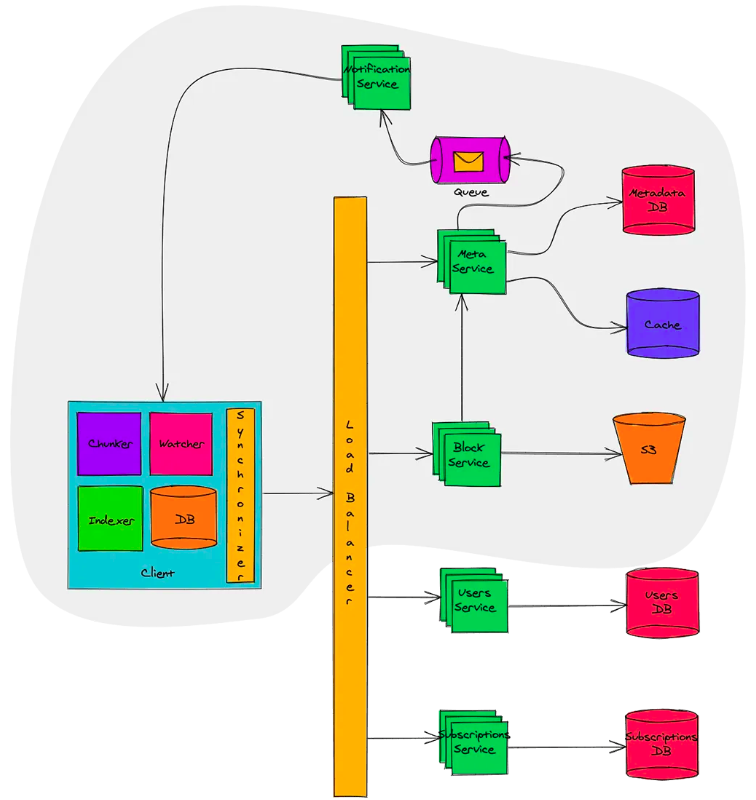
\includegraphics[width=0.8\textwidth]{img/architecture.png}
  \caption{A distributed storage architecture, illustrating the interaction between various components. The client interacts with the load balancer when making requests. The load balancer distributes different requests to the metadata service, block service, and database. The metadata service manages the metadata and interacts with the notification service to send updates. The block service handles the actual data storage and retrieval, while the database stores structured data related to the system's operation and user credentials. The notification service provides real-time updates to clients and other components. [Source: \cite{Dropbox_solution2}]}\label{fig:architecture}
\end{figure}


\section{Client}
The \textbf{Client} is the primary interface through which users interact with the storage system. It can be implemented in multiple forms:
\begin{itemize}
    \item \textbf{APIs and Protocols:} Clients may use HTTP, gRPC, or other APIs to communicate with the storage backend. For example, a developer might use RESTful APIs to integrate the storage service into their application.
    \item \textbf{Web Interface:} End users can interact with the system via a browser-based interface, providing ease of access and management.
    \item \textbf{Daemon Processes:} Applications like Dropbox use background daemon processes to monitor file system changes. This process automatically synchronizes files across devices by detecting updates and uploading or downloading files as needed.
\end{itemize}
\textbf{Example:} When a user modifies a file on their computer, the client-side daemon detects this change and triggers an upload request via the API, ensuring that the most current version is stored and replicated across devices.

\section{Frontend Server}
The \textbf{Frontend Server} acts as the gateway to the distributed storage system. Its responsibilities include:
\begin{itemize}
    \item \textbf{Handling Client Requests:} It receives and processes incoming requests, authenticating and authorizing users.
    \item \textbf{Session Management:} It maintains session states to ensure that client interactions remain consistent and secure.
    \item \textbf{Request Routing:} It forwards requests to the appropriate backend components, such as storage or metadata services.
\end{itemize}
\textbf{Example:} In a cloud storage platform, the frontend server might receive an HTTP request to upload a file. It then validates the user session, checks permissions, and routes the request to the backend servers responsible for handling the file storage.

\section{Metadata Service}
The \textbf{Metadata Service} is critical for managing the information about the stored data:
\begin{itemize}
    \item \textbf{Metadata Storage:} It holds metadata such as file size, creation date, permissions, and file block information.
    \item \textbf{Access Control:} Metadata is used to enforce security policies and access rights.
    \item \textbf{System Scalability:} By efficiently managing metadata, the system can quickly locate and retrieve data blocks, which is essential for large-scale storage environments.
\end{itemize}
\textbf{Example:} In the Hadoop Distributed File System (HDFS), the NameNode functions as the metadata service, tracking where each block of data is stored across the cluster.

\section{Notification Service}
The \textbf{Notification Service} provides real-time communication between components:
\begin{itemize}
    \item \textbf{Asynchronous Messaging:} It sends alerts, status updates, or error notifications to various services.
    \item \textbf{Client Updates:} It can notify clients about changes, such as the status of file block uploads or replication progress.
\end{itemize}
\textbf{Example:} When a large file is being split and distributed across several storage nodes, the notification service can update the client on the progress, ensuring transparency and timely error handling if issues arise.

\section{Block Service}
The \textbf{Block Service} is responsible for the physical storage and management of data blocks:
\begin{itemize}
    \item \textbf{Data Chunking:} Large files are split into manageable blocks, which are stored separately to improve retrieval efficiency and fault tolerance.
    \item \textbf{Redundancy and Replication:} To ensure high availability, blocks are often replicated across multiple nodes.
\end{itemize}
\textbf{Example:} In systems like Amazon S3 or HDFS, the block service handles the distribution and replication of file chunks, ensuring that data remains accessible even if one node fails.

\section{Database}
The \textbf{Database} component stores structured data related to the system's operation:
\begin{itemize}
    \item \textbf{Structured Data Management:} This includes information such as user credentials, access logs, and configuration settings.
    \item \textbf{Distributed Databases:} To achieve high availability and scalability, databases in distributed systems are often replicated across nodes.
    \item \textbf{Types:} Both SQL (e.g., MySQL, PostgreSQL) and NoSQL (e.g., Cassandra, MongoDB) databases are employed based on the use-case requirements.
\end{itemize}
\textbf{Example:} A metadata repository may use a NoSQL database for rapid query performance and horizontal scaling, while a transactional logging system might rely on a relational SQL database for ACID-compliant operations.

\section{Load Balancer}
The \textbf{Load Balancer} distributes network traffic evenly across multiple servers:
\begin{itemize}
    \item \textbf{Traffic Distribution:} It prevents any single server from becoming a bottleneck by spreading out incoming requests.
    \item \textbf{Fault Tolerance:} In case one server goes down, the load balancer redirects traffic to healthy servers.
    \item \textbf{Algorithms:} Common strategies include round-robin, least connections, and IP hash.
\end{itemize}
\textbf{Example:} A load balancer might be used to distribute client requests across several frontend servers, ensuring that no single server becomes overwhelmed during peak usage times.

\section{Message Queues}
\textbf{Message Queues (MQ)} enable asynchronous communication between distributed system components:
\begin{itemize}
    \item \textbf{Decoupling Services:} They allow different parts of the system to operate independently by queuing messages for later processing.
    \item \textbf{High Throughput:} MQs are designed to handle large volumes of messages efficiently.
    \item \textbf{Common Technologies:} Examples include RabbitMQ, Apache Kafka, and Amazon SQS.
\end{itemize}
\textbf{Example:} In a distributed storage system, a message queue can handle tasks like file processing and replication requests, ensuring that these tasks are processed in an orderly and fault-tolerant manner.

\section{Cache}
A \textbf{Cache} is a high-speed data layer used to store frequently accessed data:
\begin{itemize}
    \item \textbf{Latency Reduction:} Caches help reduce the time required to access data, thereby improving overall system performance.
    \item \textbf{Resource Optimization:} By storing temporary data, caches help reduce the load on backend systems.
    \item \textbf{Technologies:} Common caching solutions include Redis and Memcached.
\end{itemize}
\textbf{Example:} Frequently accessed metadata or small file fragments might be stored in a Redis cache, ensuring that user queries are served rapidly without repeatedly accessing slower backend storage.
 % Understand basic architectures for implementing such systems. high level
\chapter{Tectonic File System by Meta}\label{chap:tectonic}

Tectonic\cite{tectonic} is Meta's distributed file system designed for internal use. Each Tectonic cluster serves roughly ten tenants—distinct internal systems that do not share data—with varying requirements and workloads. As a general-purpose file system, Tectonic is built to support a wide range of applications, from low-latency operations to high-throughput and large-scale storage needs.

\section{Motivation}\label{sec:tectonic_motivation}
Before Tectonic, Meta deployed several specialized file systems to address different workload needs for different needs. For example, Haystack\cite{haystack} and F4\cite{f4} were used for BLOB (Binary Large Object) storage. Haystack was used for hot BLOBs, which are frequently accessed and require low latency, while F4 was used for warm BLOBs, which are accessed less frequently and can tolerate higher latency. Moreover the amount of data stored in F4 was significantly larger than that in Haystack. This particular approach of using seprate file systems for different workloads led to inefficient resource usage. Hot BLOBs in Haystack needed high IOPS but would not use the full capacity of the storage nodes, while warm BLOBs in F4 required high disk storage capacity but would not use the full IOPS capacity of the storage nodes. This resulted in underutilization of the surplus resources in the system. The idea was to use a single file system that could handle all workloads, allowing for better resource utilization and management.

On the other hand, HDFS\cite{hdfs} was employed for data warehouse workloads that required high throughput and large storage volumes. The HDFS clusters were limited in size due to a single NameNode, which could not scale to the required size and required using multiple clusters which would add its own operational overhead. Indeed, there was a need for a design that could scale to exabyte levels.

\section{Challenges}\label{sec:tectonic_challenges}
Designing a general-purpose file system like Tectonic introduces several challenges:
\begin{itemize}
    \item \textbf{Performance Isolation:} Ensuring that the workload of one tenant does not negatively impact the performance of another, while still allowing surplus resources to be shared.
    \item \textbf{Scaling to Exabyte Scale:} Efficiently managing metadata for exabyte-scale storage while also being able to provide fast access.
    \item \textbf{Multi-tenancy:} Providing a flexible design that accommodates tenant-specific optimizations without compromising the overall system performance.
\end{itemize}

\section{Design of Tectonic}
We first discuss the overall architecture of Tectonic, followed by its multitenancy features which enable the system to support multiple tenants with surplus resource sharing. We then explore the access control mechanisms and tenant-specific optimizations that enhance performance for specific workloads. 

\subsection{Tectonic Architecture}\label{sec:tectonic_architecture}

A Tectonic cluster is composed of \textbf{Chunk Stores}, \textbf{Metadata Stores}, and \textbf{Background Services}. A \textbf{Client Library}, tailored for various Tectonic use cases, interfaces with the Metadata and Chunk Stores to store and retrieve data. The architecture of Tectonic is illustrated in \Cref{fig:tectonic_architecture}, with additional details provided in the subsequent sections. Tectonic clusters are resilient to host, rack, and power failures at the data center level. For geo-replication, tenants can deploy multiple Tectonic clusters across different data centers.

\begin{figure}[htbp]
    \centering
    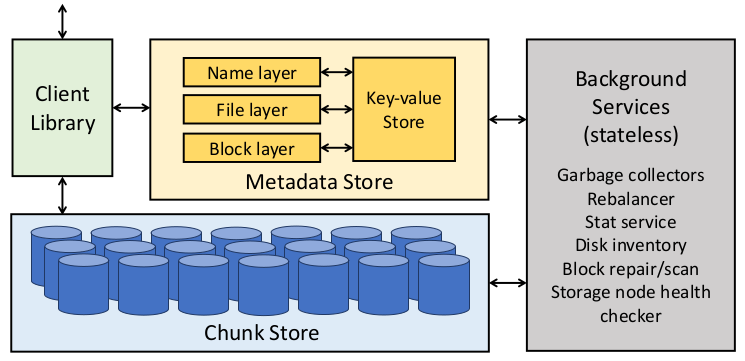
\includegraphics[width=0.8\textwidth]{img/tectonic.png}
    \caption{Tectonic architecture, with arrows indicating network calls. File system metadata is stored in a key-value store. All components are stateless, except for the Chunk and Metadata Stores. [Source: \cite{tectonic}].}
    \label{fig:tectonic_architecture}
\end{figure}

\subsubsection{Chunk Store}\label{sec:chunk_store}
In Tectonic, a file is composed of multiple blocks, each containing several chunks, which are the fundamental data storage unit. The Chunk Store is a flat, distributed object store that manages these chunks and is designed to scale linearly with the number of storage nodes, supporting exabytes of data. This abstraction is managed by the Client Library and the Metadata Store, which handle higher-level abstractions like blocks and files.

Chunks are stored as files on storage nodes, each running a local instance of XFS. These nodes are equipped with 36 hard drives for chunk storage and a 1 TB SSD for XFS metadata and caching frequently accessed chunks. The SSD cache is managed using a flash endurance-aware caching library to optimize performance. Tectonic ensures block durability through \textbf{Reed-Solomon (RS)}\cite{ReedSolomon} encoding or replication. Chunks within blocks are distributed across fault domains for fault tolerance, and background services repair damaged or lost chunks to maintain data durability.

\subsubsection{Metadata Store}\label{sec:metadata_store}
Tectonic addresses the challenge of managing large volumes of metadata by organizing it hierarchically into multiple layers. The Metadata Store is a distributed key-value store, divided into three distinct layers:

\begin{itemize}\label{list:metadata_layers}
    \item \textbf{Name Layer}: Maps directories to the sub-directories and files they contain.
    \item \textbf{File Layer}: Maps files to their associated blocks.
    \item \textbf{Block Layer}: Maps blocks to their corresponding chunks and includes a reverse mapping from chunks to blocks, which aids in garbage collection.
\end{itemize}

Unlike traditional directory mappings where a key maps to a list of values, Tectonic stores keys in an expanded format to enable faster updates. For example, if directory \texttt{A} contains sub-directory \texttt{B} and file \texttt{C}, the keys stored will be \texttt{(A, B)} and \texttt{(A, C)}, rather than a single key \texttt{A} mapping to a list containing \texttt{B} and \texttt{C}. This approach accelerates updates and eliminates the need for locks during the update process. However, listing the contents of a directory requires a prefix scan over the keys.

Another design choice is the use of \textbf{hash partitioning} for the different layers, instead of range partitioning. This method provides better load balancing and helps prevent hotspots in the system, particularly for Data Warehouse parallel processing workloads.

At a lower level, the Metadata Store is powered by ZippyDB \cite{zippydb}, with each node using RocksDB \cite{rocksdb} for storing key-value pairs. Fault tolerance is ensured through replication, utilizing the Paxos consensus protocol \cite{paxos}.

While this design enables scalability and mitigates hotspots, it introduces some challenges. The layered architecture results in increased latency for metadata operations. To address this, Tectonic clients can seal directories, which allows for caching of metadata within the client library. Furthermore, Tectonic does not support atomic cross-directory operations, nor does it provide a direct API for listing the entire contents of a directory. Consequently, clients are required to implement a wrapper around the list API to retrieve the contents of a directory.


\subsubsection{Client Library} \label{sec:client_library}

The Client Library provides a filesystem abstraction using the metadata, operating at the chunk granularity for read and write operations. It enforces \textbf{Single Writer Semantics} by issuing a token when a client opens a file for appending. This token must accompany all subsequent metadata updates, ensuring that only the last process to open the file can perform writes.

For multiple-writer semantics, tenants can implement custom serialization protocols on top of Tectonic. Since the filesystem is intended for internal clients, such protocols are manageable and can be handled by the organization's developers using Tectonic for their specific use cases.


\subsubsection{Background Services} \label{sec:background_services}

Background services ensure consistency, durability, and efficient data management in Tectonic. These services maintain metadata consistency between layers, repair lost data, rebalance storage across nodes, and handle rack drains. They also publish statistics on filesystem usage.

The background services operate on one shard at a time, similar to the Metadata Store. Key services include a garbage collector that cleans up metadata inconsistencies (e.g., caused by failed Client Library operations or lazy object deletion), and a rebalancer and repair service that work together to relocate or delete chunks. The rebalancer identifies chunks needing relocation due to events like hardware failures or increased storage capacity, while the repair service handles the actual data movement, operating on a per-Block layer shard and per-disk basis to scale horizontally. The block layer and the rebalancer service work together to ensure that the total number of copysets\cite{copyset} is maintained, and that chunks are distributed evenly across nodes. 

A copyset refers to a group of replicas of a data chunk stored across different nodes. The system ensures that each chunk of data has multiple copies distributed across multiple nodes to protect against node failures. The copyset concept ensures that even in the event of hardware or network failures, data availability and durability are maintained by limiting the total number of distinct copysets in the system. Each chunk belongs to a specific copyset, and the number of replicas (copysets) is dynamically managed based on system requirements such as redundancy levels, storage capacity, and load balancing.


\subsection{Multitenancy}\label{sec:multitenancy}

Tectonic categorizes resources into two types: \textbf{non-ephemeral} and \textbf{ephemeral}. Non-ephemeral resources change slowly over time and typically do not have dynamic adjustment semantics. An example of this is the storage capacity allocated to a tenant, which is pre-configured and remains static.

In contrast, ephemeral resources change rapidly and require dynamic monitoring and automated adjustments. Examples include storage IOPS capacity and metadata query capacity.

One key challenge is determining the appropriate level at which to manage resources. Providing isolation at the application level is complex due to the difficulty of managing resources across multiple applications. On the other hand, isolation at the tenant level may be too generalized. To address this, Tectonic introduces the concept of \texttt{TrafficGroup} and \texttt{TrafficClass} for managing resources. A \texttt{TrafficGroup} consists of applications with similar storage requirements within a tenant, and each \texttt{TrafficGroup} is assigned a \texttt{TrafficClass}. Tectonic defines three types of \texttt{TrafficClass}: \texttt{Gold} (Latency-sensitive), \texttt{Silver} (Normal), and \texttt{Bronze} (Background services). Tectonic manages resource access both at the global level and per node.

\subsubsection{Global Resource Management}\label{sec:global_resource_management}

The goal of global resource management is twofold: to limit resource usage and to efficiently share surplus resources across tenants. To achieve this, Tectonic employs a modified version of the leaky bucket algorithm, utilizing high-performance, near-real-time distributed counters.

The resource management process works as follows:

\begin{itemize}\label{list:resource_management}
    \item A resource counter is incremented for the corresponding \texttt{TrafficGroup} whenever a resource is used.
    \item If spare capacity is available, it is allocated for use.
    \item If a tenant exceeds its allocated capacity, the system checks for surplus capacity within other \texttt{TrafficGroups} of the same tenant.
    \item If no surplus capacity is found, the system then checks for spare capacity in other tenants.
\end{itemize}

When sharing resources between \texttt{TrafficGroups}, the request is treated as the \texttt{TrafficClass} of the lower-priority group. For example, if a \texttt{Gold} \texttt{TrafficGroup} requests resources from a \texttt{Silver} \texttt{TrafficGroup}, the request is treated as \texttt{Silver}. This prevents excessive increases in high-priority traffic, ensuring that the system remains stable and that many \texttt{Gold} requests can still meet their requirements.

\subsubsection{Per-Node Resource Management}\label{sec:per_node_resource_management}

The aim of per-node resource management is to prevent hotspots and ensure that the latency requirements for high-priority traffic, such as \texttt{Gold} class traffic, are met.

To achieve this, a Weighted Round-Robin (WRR) scheduling approach is employed. In this scheme, a request is skipped if its quota has already been used or if granting it would exceed the quota.

Several optimizations are applied to improve resource utilization:

\begin{itemize}
    \item Lower-priority request classes can yield their turn to higher-priority requests if there will still be enough time to service the lower-priority requests afterward.
    \item The number of non-\texttt{Gold} traffic requests in the queue for a disk is limited if there are pending \texttt{Gold} requests.
    \item Disks may rearrange requests to prioritize higher-priority traffic. If a \texttt{Gold} request is pending for a certain threshold amount of time, non-\texttt{Gold} requests may be deferred to prioritize the \texttt{Gold} request.
\end{itemize}

It is important to note that resource sharing at the node level is unnecessary, as it has already been handled globally.

\subsubsection{Access Control}\label{sec:access_control}

Tectonic employs a token-based access control mechanism to ensure that only authorized clients can access the system. In this system, each layer generates a token that must be included in subsequent requests to the next layer. The token is piggybacked on the request-reply. This mechanism effectively controls access by verifying the presence of a valid token in each request.

\subsection{Tenant-Specific Optimizations}\label{sec:tenant_specific_optimizations}

As mentioned in \Cref{sec:client_library}, the client library communicates directly with the chunk stores at the chunk granularity. This approach enables the optimization of read and write operations for specific tenants.

\subsubsection{Data Warehouse Write Optimizations}\label{sec:data_warehouse_optimization}

Data Warehouse storage has read after complete write semantics that is data is only read after the write operation is complete. This allows for optimizations such as: 

\subsubsection*{Asynchronous Writes}\label{sec:asynchronous_writes}

To optimize write operations, applications buffer writes until enough data is accumulated to form a block of the desired size. RS-Encoding is then done at the client itself, reducing the amount of data that needs to be transmitted to different nodes. This approach also reduces the number of network calls and disk seeks, enhancing write performance.

Importantly, there is no inconsistency introduced because metadata is only updated after the complete write operation has been successfully finished. This approach guarantees that data consistency is maintained throughout the write process.

\subsubsection*{Hedged Quorum Writes}\label{sec:hedged_quorum_writes}

Hedged quorum writes aim to improve write latency by sending reservation requests to more nodes than the minimum required for a successful operation. Rather than waiting for the write to complete on all nodes, the system only waits until a majority of blocks have been successfully written, at which point the client is notified. 

This method effectively reduces the 99th percentile latency, enhancing the system's responsiveness and providing faster acknowledgment to clients.

\subsubsection{Blob Storage Optimizations}\label{sec:blob_storage_optimization}

\subsubsection*{Consistent Partial Block Appends}\label{sec:consistent_partial_block_appends}

To optimize append operations in blob storage, the system ensures that appends are consistent by waiting until the quorum size of appends is reached. This ensures data integrity and reduces unnecessary writes. Additionally, only the block creator is allowed to perform append operations, maintaining consistency and preventing data corruption.

Once an append operation is completed, the metadata is updated with the post-append block size and its corresponding checksum, ensuring consistency and reliability in the storage system.

\subsubsection*{Reencoding Blocks for Storage Efficiency}\label{sec:reencoding_blocks}

Reencoding blocks for storage efficiency is made possible by the Client Library-driven design. Unlike traditional file systems, which typically require preconfiguration for file storage, this design allows more flexibility in optimizing storage. Specifically, blocks are reencoded from replicated formats to Reed-Solomon (RS) after a certain amount of time has passed. This process reduces the storage overhead associated with replication, enhancing storage efficiency and reducing costs.

\subsection{Conclusion}\label{sec:tectonic_conclusion}
As Tectonic is designed for Meta's internal use, it does not implement many of the semantics required by clients. Instead, it leaves these responsibilities to developers, who are expected to implement them at a higher level while using Tectonic. This design choice allows Tectonic to be more efficient and flexible while still meeting the needs of its users. As a result, Tectonic is able to provide a general-purpose file system that can handle a wide range of workloads and applications, making it a valuable asset for Meta's internal operations. % Study practical implementation 1.
\chapter{Dropbox}\label{chap:dropbox}

\section{Motivation and Background}
Dropbox was born out of a simple yet pervasive frustration: the hassle of accessing files on multiple devices. The idea took shape when co-founder Drew Houston repeatedly forgot his USB drive—a common inconvenience that highlighted a broader need for seamless file synchronization and remote access \cite{BusinessInsider2018}.

Inspired in part by the efficient file access model of MIT’s Athena system, which enabled students to retrieve files from any campus workstation, Houston envisioned a system that brought similar convenience to the general public. Thus, Dropbox emerged as an innovative cloud storage solution aimed at eliminating the dependency on physical storage devices \cite{Awfis2021}.

\section{Key Problems Addressed}
\subsection{Challenges Before Dropbox}
\begin{itemize}
    \item \textbf{Reliance on Physical Storage:} Users had to carry USB drives or email files to themselves, which was not only inconvenient but also prone to loss or damage.
    \item \textbf{File Versioning Issues:} Maintaining the latest version of a file across various devices, especially during collaborations, was a persistent challenge.
    \item \textbf{Unreliable Existing Tools:} Early file-syncing tools were often buggy, slow, and required extensive manual configuration.
    \item \textbf{Limited Remote Access:} Accessing files from remote locations typically involved cumbersome methods, reducing overall productivity.
\end{itemize}

\subsection{Dropbox's Innovative Solutions}
\begin{itemize}
    \item \textbf{Automatic File Synchronization:} Files are updated in real time across all connected devices, ensuring users always work with the latest version.
    \item \textbf{Cloud Storage Infrastructure:} By storing files remotely, Dropbox minimizes the risk of data loss from hardware failures.
    \item \textbf{Robust Version Control:} Users can effortlessly recover previous versions of their files, which is invaluable during collaborative projects.
    \item \textbf{User-Friendly Interface:} An intuitive drag-and-drop functionality makes file management simple and integrates seamlessly with existing file systems.
    \item \textbf{Enhanced Collaboration:} Shared folders and real-time updates foster smoother teamwork, eliminating the need for repetitive file transfers.
\end{itemize}


\section{Challenges}
Dropbox-like systems face several unique challenges that stem from their core mission to provide seamless, efficient, and secure file synchronization across a variety of devices. Some of these challenges include:

\begin{enumerate}
    \item \textbf{High Read-to-Write Ratio (~1:1):} With continuous synchronization across multiple devices, Dropbox experiences nearly as many reads as writes, necessitating efficient caching and deduplication mechanisms 
    \item \textbf{Conflict Resolution in Synchronization:} Efficiently managing version conflicts when multiple users edit the same file is crucial to prevent data loss and ensure a smooth user experience 
    \item \textbf{Efficient Metadata Storage:} With millions of files per user, optimizing metadata storage and retrieval is vital for maintaining performance.
    \item \textbf{Eventual Consistency vs. Strong Consistency:} To ensure smooth synchronization, Dropbox prioritizes eventual consistency, which may lead to temporary file discrepancies 
    \item \textbf{Efficient Data Deduplication:} Storing only one copy of identical files or blocks helps reduce storage costs and improves system efficiency 
    \item \textbf{Bandwidth Optimization:} Techniques such as compression, differential synchronization, and intelligent throttling are used to minimize network usage during file transfers 
    \item \textbf{Handling Offline Changes:} Detecting edits made while offline and synchronizing them accurately when the device reconnects presents unique challenges.
    \item \textbf{Delta Encoding for Efficient Transfers:} Transmitting only the byte-level differences between file versions rather than full file copies is critical for reducing data transfer volumes 
    \item \textbf{Multi-Device Conflict Handling at Scale:} Employing timestamp-based versioning and user notifications helps resolve conflicts that arise from simultaneous edits on multiple devices.
    \item \textbf{Global Namespace Management:} Preventing file path collisions and ensuring fast lookup in a distributed system is essential for maintaining a consistent user experience 
    \item \textbf{Latency Reduction in Large Folder Syncs:} Prioritizing critical files while indexing large directories in the background minimizes perceived latency during synchronization 
\end{enumerate}


\section{Architecture}
Dropbox's system architecture has evolved from a simple file synchronization model to a distributed, highly scalable, and fault-tolerant platform. This section details the evolution and technical design of both server- and client-side components.

\subsection{Initial Design}
The early architecture was based on a straightforward client-server model:
\begin{itemize}
    \item \textbf{Client Application:} Monitors local file changes and communicates with the server.
    \item \textbf{Central Server:} Stores files and manages metadata.
    \item \textbf{Full-file Synchronization:} Entire files were transmitted for each update, leading to inefficient bandwidth and storage use.
\end{itemize}

\subsection{Enhanced Server Architecture}
To meet increased demands, the backend was re-engineered into modular components, as illustrated in \Cref{fig:write-path}.

\begin{figure}[H]
    \centering
    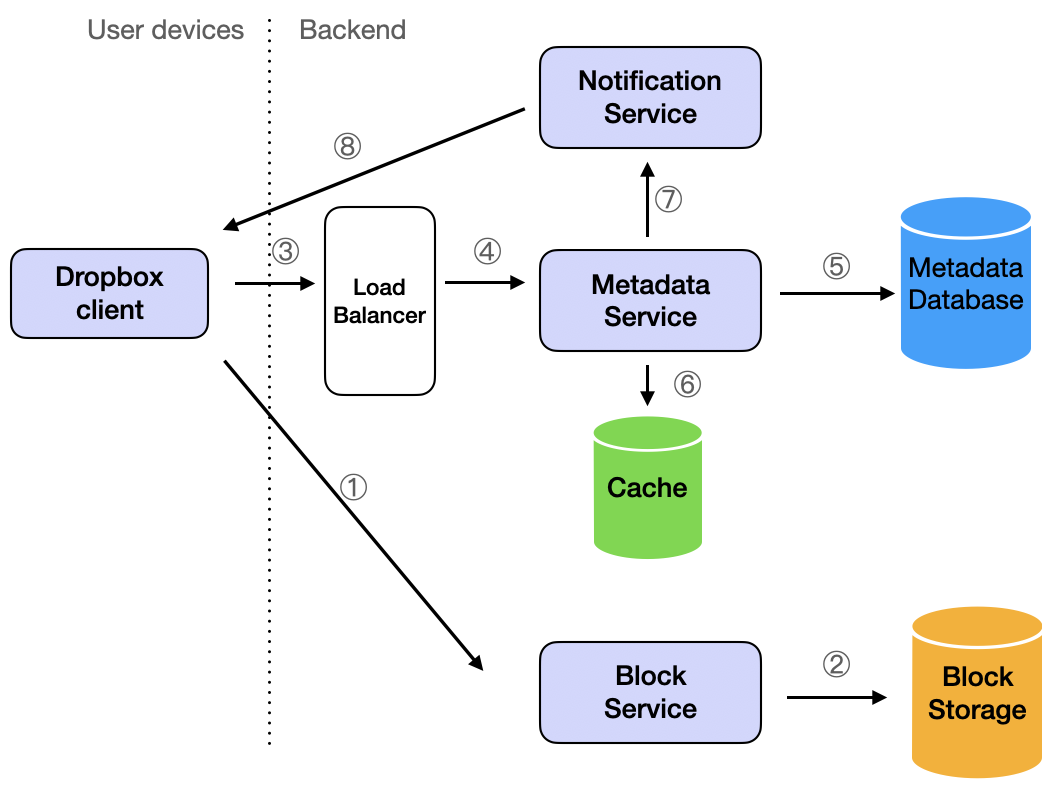
\includegraphics[width=0.8\textwidth]{img/write-path.png}
    \caption{Server-side Architecture: The Metadata Service uses a key-value store; the Block Service manages file chunks in a distributed file system; the Notification Service propagates updates; and the Load Balancer distributes client requests efficiently[Source: \cite{Dropbox_solution2}].}
    \label{fig:write-path}
\end{figure}

\subsubsection{File Chunking and Deduplication}
Files are partitioned into fixed-size 4MB chunks. Each chunk is processed with a cryptographic hash (SHA-256) to:
\begin{itemize}
    \item Uniquely identify the data block.
    \item Verify data integrity.
    \item Enable deduplication by referencing existing chunks when identical data is encountered.
\end{itemize}

\subsubsection{Block Server}
The Block Server employs a key-value storage paradigm where each SHA-256 hash acts as the key for its corresponding chunk. This design allows for rapid retrieval and minimizes redundant storage.

\subsubsection{Metadata Management}
Metadata—including file paths, versioning, and offsets—is stored in a hierarchical key-value database (e.g., LevelDB). The Metadata Service:
\begin{itemize}
    \item Synchronizes file metadata between clients and the server.
    \item Computes and disseminates incremental change sets.
    \item Interfaces with the Notification Service to propagate updates in real time.
\end{itemize}

\subsubsection{Notification Service}
A dedicated Notification Service broadcasts file update events to all subscribed clients, ensuring low-latency synchronization across devices.

\subsubsection{Load Balancing and Inter-Service Communication}
A round-robin load balancer distributes incoming requests evenly across metadata servers. Asynchronous message queues are employed to facilitate non-blocking communication between services, thereby enhancing scalability and resilience.

\subsection{Client Architecture}
Client-side improvements focus on efficient file handling and robust synchronization. \Cref{fig:client} shows the refined client workflow.

\begin{figure}[H]
    \centering
    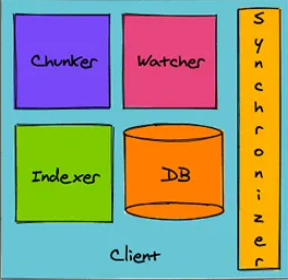
\includegraphics[width=0.4\textwidth]{img/client.png}
    \caption{Client Architecture: Integrates a file chunker, Metadata Service client, file watcher, local metadata indexer, and a synchronizer that coordinates with remote services [Source: \cite{Dropbox_solution1}].}
    \label{fig:client}
\end{figure}

\begin{enumerate}
    \item \textbf{Chunker:} Segments files into 4MB blocks for efficient block-level transmission.
    \item \textbf{Metadata Service Client:} Handles bidirectional communication with the Metadata Service to exchange change sets.
    \item \textbf{File Watcher:} Monitors local file system events and triggers indexing updates.
    \item \textbf{Indexer:} Updates the local metadata repository and notifies the synchronizer upon detecting changes.
    \item \textbf{Synchronizer:} Reconciles local state with remote services by coordinating metadata and block updates, handling both push and pull synchronization modes.
\end{enumerate}


\section{Optimizations over the Naive Approach}

\subsection{Efficient File Synchronization via DeltaSync}

DeltaSync minimizes data transfer by employing advanced delta encoding techniques that target only the modified portions of files. Its design philosophy is to reduce bandwidth usage, avoid redundant transmissions, and achieve near-real-time updates.

\subsubsection{Rolling Hash-based Content Defined Chunking (CDC)}
To overcome the limitations of fixed-size chunking (the \emph{block shift problem}), DeltaSync uses a rolling hash function to determine chunk boundaries based on file content:
\begin{enumerate}
    \item \textbf{Block Hashing:} The file is processed with a sliding window to compute a rolling hash for each tentative block.
    \item \textbf{Dynamic Boundary Detection:} A chunk boundary is defined when the hash satisfies:
    \[
        H_i \mod T = 0,
    \]
    where \(H_i\) is the current hash and \(T\) is a threshold parameter set to achieve an optimal average chunk size.
    \item \textbf{Efficient Update Mechanism:} The rolling hash is updated as:
    \[
        H_i = \Bigl( H_{i-1} - B_{i-1} \cdot P^{w-1} \Bigr) \cdot P + B_{i+w-1} \mod M,
    \]
    with:
    \begin{itemize}
        \item \(B_{i-1}\) and \(B_{i+w-1}\) as the outgoing and incoming bytes,
        \item \(P\) as a prime number,
        \item \(w\) as the window size,
        \item \(M\) as a modulus.
    \end{itemize}
\end{enumerate}

\subsubsection{Handling Insertions and Deletions}
By leveraging CDC, DeltaSync re-aligns chunk boundaries dynamically. For example:
\[
\text{Original: } [A][B][C][D][E] \quad \Longrightarrow \quad \text{Modified: } [A][B'] [X] [C][D][E],
\]
where only the affected chunks (\(B'\) and \(X\)) require retransmission.

\subsubsection{Supplementary Optimizations}
Additional technical enhancements include:
\begin{itemize}
    \item \textbf{Deduplication:} Transmitting and storing only unique chunks across files and users.
    \item \textbf{Compression:} Compressing data to further reduce transmission size.
    \item \textbf{Parallel Transfers:} Uploading multiple modified chunks concurrently to maximize throughput.
\end{itemize}

\subsection{Real-Time Notifications via Long Polling}

Long polling is employed to notify clients of file changes in near real-time while maintaining minimal resource overhead. Its core philosophy is to balance immediacy with scalability.

\subsubsection{Mechanism Overview}

Long polling maintains an open HTTP connection until a file event occurs:
\begin{enumerate}
    \item \textbf{Initiate Request:}
    \begin{lstlisting}
GET https://notify.dropboxapi.com/2/files/list_folder/longpoll?cursor=<CURSOR>&timeout=<TIMEOUT>
    \end{lstlisting}
    
    \item \textbf{Event Trigger:} If a file change occurs within the timeout period, the server responds:
    \begin{lstlisting}
{"changes": true}
    \end{lstlisting}
    
    \item \textbf{Detailed Update Retrieval:} The client then fetches specifics by posting:
    \begin{lstlisting}
POST https://api.dropboxapi.com/2/files/list_folder/continue
{ "cursor": "<CURSOR>" }
    \end{lstlisting}
    
    \item \textbf{No Update Scenario:} When no change is detected, the server replies:
    \begin{lstlisting}
{"changes": false}
    \end{lstlisting}
    prompting the client to reissue the long poll request.
\end{enumerate}

\subsubsection{Technical Advantages}
Long polling offers several benefits:
\begin{itemize}
    \item \textbf{Resource Efficiency:} Lower overhead compared to persistent connections (e.g., WebSockets).
    \item \textbf{Firewall Compatibility:} Operates seamlessly over HTTP(S), ensuring compatibility with common network configurations.
    \item \textbf{Scalability:} Designed to handle millions of concurrent clients with minimal server load.
\end{itemize}

\subsubsection{Implementation Enhancements}
Further optimizations include:
\begin{itemize}
    \item \textbf{Backoff Strategy:} Gradually increasing retry intervals during periods of inactivity.
    \item \textbf{Cursor-based State Tracking:} Maintaining synchronization state to avoid redundant updates.
    \item \textbf{Batching Notifications:} Grouping multiple file changes into single notifications to optimize network utilization.
\end{itemize}

 % Study practical implementation 2.
\chapter{Ceph Distributed Storage System}\label{chap:ceph} 
Ceph uniquely delivers object, block, and file storage in one unified system. Ceph is highly reliable, easy to manage, and free. Ceph delivers extraordinary scalability–thousands of clients accessing petabytes to exabytes of data. A Ceph Node leverages commodity hardware and intelligent daemons, and a Ceph Storage Cluster accommodates large numbers of nodes, which communicate with each other to replicate and redistribute data dynamically

\section{Motivation}\label{sec:ceph_motivation}
 Prior to Ceph, storage infrastructures were typically built using multiple specialized systems. Traditional solutions often required centralized metadata management or separate systems for block, file, and object storage—leading to inefficiencies and increased costs. The motivation behind Ceph was to consolidate these diverse storage needs into one cohesive system that:
\begin{itemize}
    \item \textbf{Delivers Unified Storage:} By integrating object, block, and file interfaces, Ceph simplifies infrastructure management.
    \item \textbf{Enhances Scalability:} Ceph is designed to scale out by using a distributed algorithm (CRUSH) for data placement, which eliminates central bottlenecks. 
    \item \textbf{Ensures High Availability:} Its self-healing and self-managing properties allow for automatic data replication and recovery, ensuring continuous operation despite hardware failures.
\end{itemize}
These goals were driven by the need for a flexible, resilient system that could serve modern cloud and big data applications without resorting to expensive, specialized hardware. \cite{cloudification2024} 

\section{Challenges}\label{sec:ceph_challenges}
Designing a distributed storage system like Ceph involves addressing several core challenges: 

\begin{itemize}
    \item \textbf{Data Placement and Scalability:} Distributing data across thousands of nodes requires a robust algorithm (such as CRUSH) that dynamically balances loads and adapts to changes in the cluster. 
    \item \textbf{Fault Tolerance and Self-Healing:} The system must detect and recover from node or disk failures automatically, ensuring data durability without manual intervention. 
    \item \textbf{Performance Optimization:} Achieving high throughput and low latency across a network of commodity hardware is complex, especially when replicating or erasure-coding data. 
    \item \textbf{Heterogeneous Hardware Support:} Supporting a mix of storage devices (HDDs, SSDs, NVMe) while maintaining consistent performance requires careful tuning and design. 
    \item \textbf{Management Complexity:} The distributed nature of the system introduces challenges in configuration, monitoring, and scaling, all of which must be simplified for operational efficiency. 
\end{itemize}

\section{Ceph Architecture}

\subsection{Core Components}

Ceph's architecture is built around the following key components:

\begin{itemize}
    \item \textbf{Object Storage Device (OSD) Daemons}: These are the primary storage nodes responsible for storing and replicating data. Each OSD runs as a separate daemon on a physical or virtual storage device.
    \item \textbf{Monitors (MONs)}: MONs maintain the cluster map and manage metadata, ensuring that all clients and OSDs have a consistent view of the system.
    \item \textbf{Managers (MGRs)}: A Ceph Manager serves as an endpoint for monitoring, orchestration, and plug-in modules.
    \item \textbf{Metadata Servers (MDSs)}: Used for CephFS, these servers handle file system metadata and allow POSIX-compliant access to data.
\end{itemize}

Storage cluster clients and Ceph OSD Daemons use the CRUSH algorithm to compute information about the location of data. By using the CRUSH algorithm, clients and OSDs avoid being bottlenecked by a central lookup table. \cite{ceph_architecture}

\subsection{Cluster Maps and Topology Changes}

Ceph's architecture relies on various maps to represent the cluster's state:

\begin{itemize}
    \item \textbf{Monitor Map}: Lists all active MONs.
    \item \textbf{OSD Map}: Details all OSDs and their statuses.
    \item \textbf{Placement Group (PG) Map}: Describes the distribution of PGs across OSDs.
    \item \textbf{CRUSH Map}: Defines the data placement rules using the CRUSH algorithm, determining how data is distributed across the cluster.
\end{itemize}

When the cluster topology changes, such as adding or removing OSDs, these maps are updated to reflect the new state, ensuring that data placement and access remain consistent.

\subsection{Data Storage Workflow}

Ceph organizes data through a hierarchical structure:

\begin{enumerate}
    \item \textbf{Files}: User data is initially in file form.
    \item \textbf{Objects}: Files are divided into objects for storage.
    \item \textbf{Pools}: Objects are grouped into pools, which are logical collections that manage replication and placement rules.
    \item \textbf{Placement Groups (PGs)}: Pools are subdivided into PGs, which act as intermediaries to distribute objects evenly across OSDs.
    \item \textbf{OSDs}: PGs map to OSDs where the actual data resides.
\end{enumerate}

This structure ensures efficient data distribution and management within the cluster.

\subsection{Role of Placement Groups}

Placement Groups aggregate objects into manageable units, facilitating balanced data distribution and simplifying replication processes. By mapping multiple objects to a single PG, Ceph reduces the complexity of tracking individual object locations, enhancing scalability and performance.
\begin{enumerate}
    \item \textbf{Efficient Data Management}: By grouping objects, PGs reduce the complexity of tracking individual objects, enhancing performance.
    \item \textbf{Optimized Data Distribution and Recovery}: PGs enable even data distribution across OSDs. In case of an OSD failure, entire PGs can be replicated or moved, ensuring swift recovery and data integrity.
\end{enumerate}

\begin{figure}[h]
    \centering
    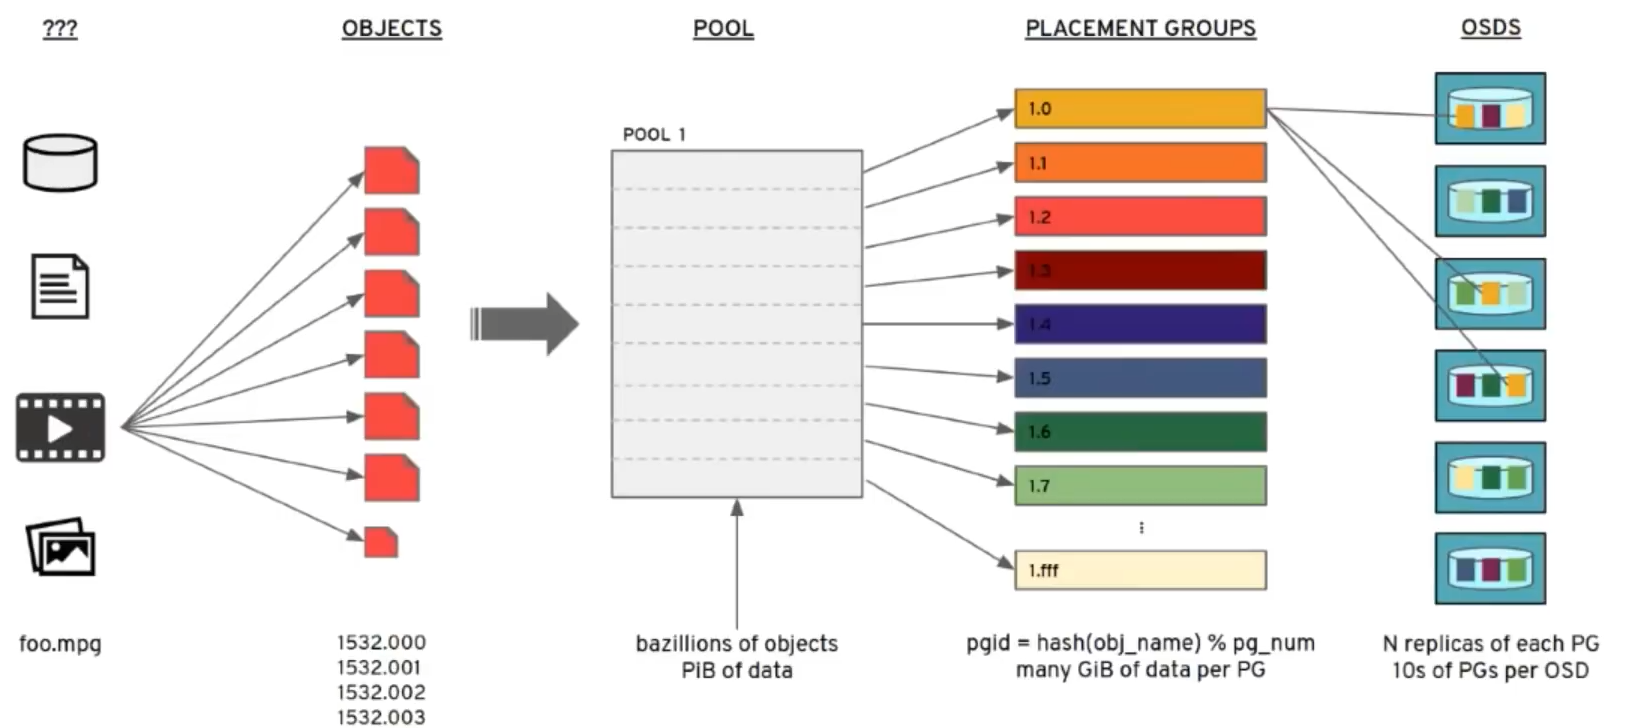
\includegraphics[width=0.8\textwidth]{img/obj_pg_osd.png}
    \caption{Relation between File, Objects, Placement Groups and OSDs. Source:  \cite{ceph_intro_video}.} 
    \label{fig:obj_pg_osd}
\end{figure}

\subsection{Data Protection Mechanisms}

Ceph employs two primary methods to ensure data durability:
\begin{itemize}
    \item \textbf{Replication}: Each object is copied to multiple OSDs based on predefined replication factors. This approach ensures data availability even if some OSDs fail.
    \item \textbf{Erasure Coding}: Data is split into chunks and encoded with redundancy information. This method provides fault tolerance with reduced storage overhead compared to replication.
\end{itemize}
\begin{figure}[h]
    \centering
    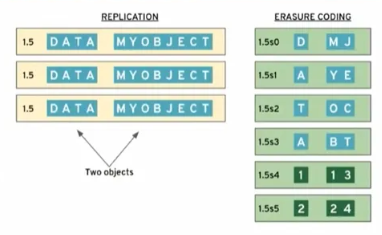
\includegraphics[width=0.7\textwidth]{img/replication_erasure_coding.png}
    \caption{Comparison of replication and erasure coding techniques \cite{ceph_intro_video}.}
    \label{fig:replication_erasure}
\end{figure}

  

\subsection{RADOS Gateway (RGW)}

The RGW is an object storage interface that provides RESTful APIs compatible with Amazon S3 and OpenStack Swift, enabling applications to interact with Ceph's object storage seamlessly.

\subsection{RGW Federation and Geo-Replication}

To enhance scalability and disaster recovery, Ceph's RGW supports:

\begin{itemize}
    \item \textbf{Federation}: Distributes the workload across multiple zones, allowing for scalable and efficient data access.
    \item \textbf{Geo-Replication}: Asynchronously replicates data across geographically dispersed clusters, ensuring data availability and disaster recovery.
\end{itemize}

\subsection{Metadata Server (MDS)}

For the Ceph File System (CephFS), the MDS manages metadata operations, such as directory structures and file attributes. This separation of data and metadata operations allows Ceph to handle high metadata workloads efficiently, providing POSIX-compliant file system access.
 % Study practical implementation 3.
\chapter{Conclusion}\label{chap:conclusion}

In this report, we  examined three distinct distributed storage systems: \textbf{Tectonic}, \textbf{Dropbox}, and \textbf{Ceph}. Although they serve different audiences and have unique design goals, their architectures offer valuable insights into the trade-offs and challenges in building scalable, fault-tolerant storage systems.

\section{Design Choices}
\begin{itemize}
    \item \textbf{Tectonic:} Developed for internal use at Meta, Tectonic emphasizes multi-tenancy and efficient resource sharing. Its layered metadata store, token-based access control, and client-side optimizations enable effective handling of large-scale, heterogeneous workloads.
    \item \textbf{Dropbox:} Designed for consumer file synchronization, Dropbox employs a client-server architecture that leverages file watchers, delta encoding, and long-polling for real-time notifications. These choices ensure low-latency updates and robust version control across multiple devices.
    \item \textbf{Ceph:} An open-source solution that unifies object, block, and file storage, Ceph is built for scalability and resilience. Its decentralized architecture, driven by the CRUSH algorithm for data placement along with replication and erasure coding, provides high availability and self-healing capabilities.
\end{itemize}

\section{Differences in Models}
The three systems illustrate different approaches to addressing the fundamental challenges of distributed storage:
\begin{itemize}
    \item \textbf{Architectural Models:} Tectonic uses a layered, tenant-focused model while Dropbox relies on a centralized client-server approach optimized for real-time synchronization. In contrast, Ceph adopts a decentralized design that eliminates single points of failure.
    \item \textbf{Consistency and Performance:} Dropbox opts for eventual consistency to facilitate rapid file synchronization, whereas Tectonic and Ceph are designed to balance strong consistency with performance, adapting their strategies based on workload and system scale.
    \item \textbf{Resource Management:} Tectonic demonstrates sophisticated resource optimization through multi-tenancy and dynamic resource sharing, while Ceph shows how decentralization and intelligent data placement can maintain performance under heavy load.
\end{itemize}

\section{Lessons Learned}
From a distributed systems perspective, the analysis of these systems offers several key takeaways:
\begin{itemize}
    \item \textbf{Trade-offs in Consistency:} The choice between strong and eventual consistency impacts system design, performance, and user experience.
    \item \textbf{Scalability and Fault Tolerance:} Decentralized approaches, as seen in Ceph, highlight the benefits of eliminating bottlenecks and ensuring data remains accessible even under failures.
    \item \textbf{Application-Specific Optimization:} Tectonic and Dropbox illustrate that system design can be tailored to meet specific use cases—whether it is internal resource management or consumer-oriented file synchronization.
\end{itemize}
Overall, these systems reflect the diverse strategies available for tackling the inherent challenges of distributed storage. Their design choices provide a rich basis for understanding how to optimize for scalability, performance, and reliability in distributed environments.


\bibliographystyle{plainurl}
\bibliography{references}

\end{document}
